% !TEX encoding = UTF-8
% !TEX TS-program = pdflatex
% !TEX root = ../Articolo.tex
% !TEX spellcheck = it-IT

%************************************************
\section{DEM Characterization Workflow Powder}
\label{section:Demcharacterizationworkflowpowder}
%************************************************

The powder characterization has not been exstensively studied yet in our lab (at least my knowledge).
Just a prototype of colliding hollow sphere was conceived, but the results had not been analyzed nor evaluated.\\

\subsection{Hollow spheres}
\label{subsection:hollowspheres}

The experimental apparatus can be seen in Figure \ref{fig:007hollowspheredevice2}. The main components are two twin aluminum spheres, independently connected via U-shaped steel structures to rotating beams. The rotation of the beams, and so the angular speed of the spheres, is registered by a couple of angle-meters.\\
The spheres are hollow, particles can be inserted inside, and the \ac{ra} is 50 millimeters.\\

\begin{figure}[!h]
\centering
\subfloat[HS experimental device]
{\label{fig:007hollowspheredevice2}%
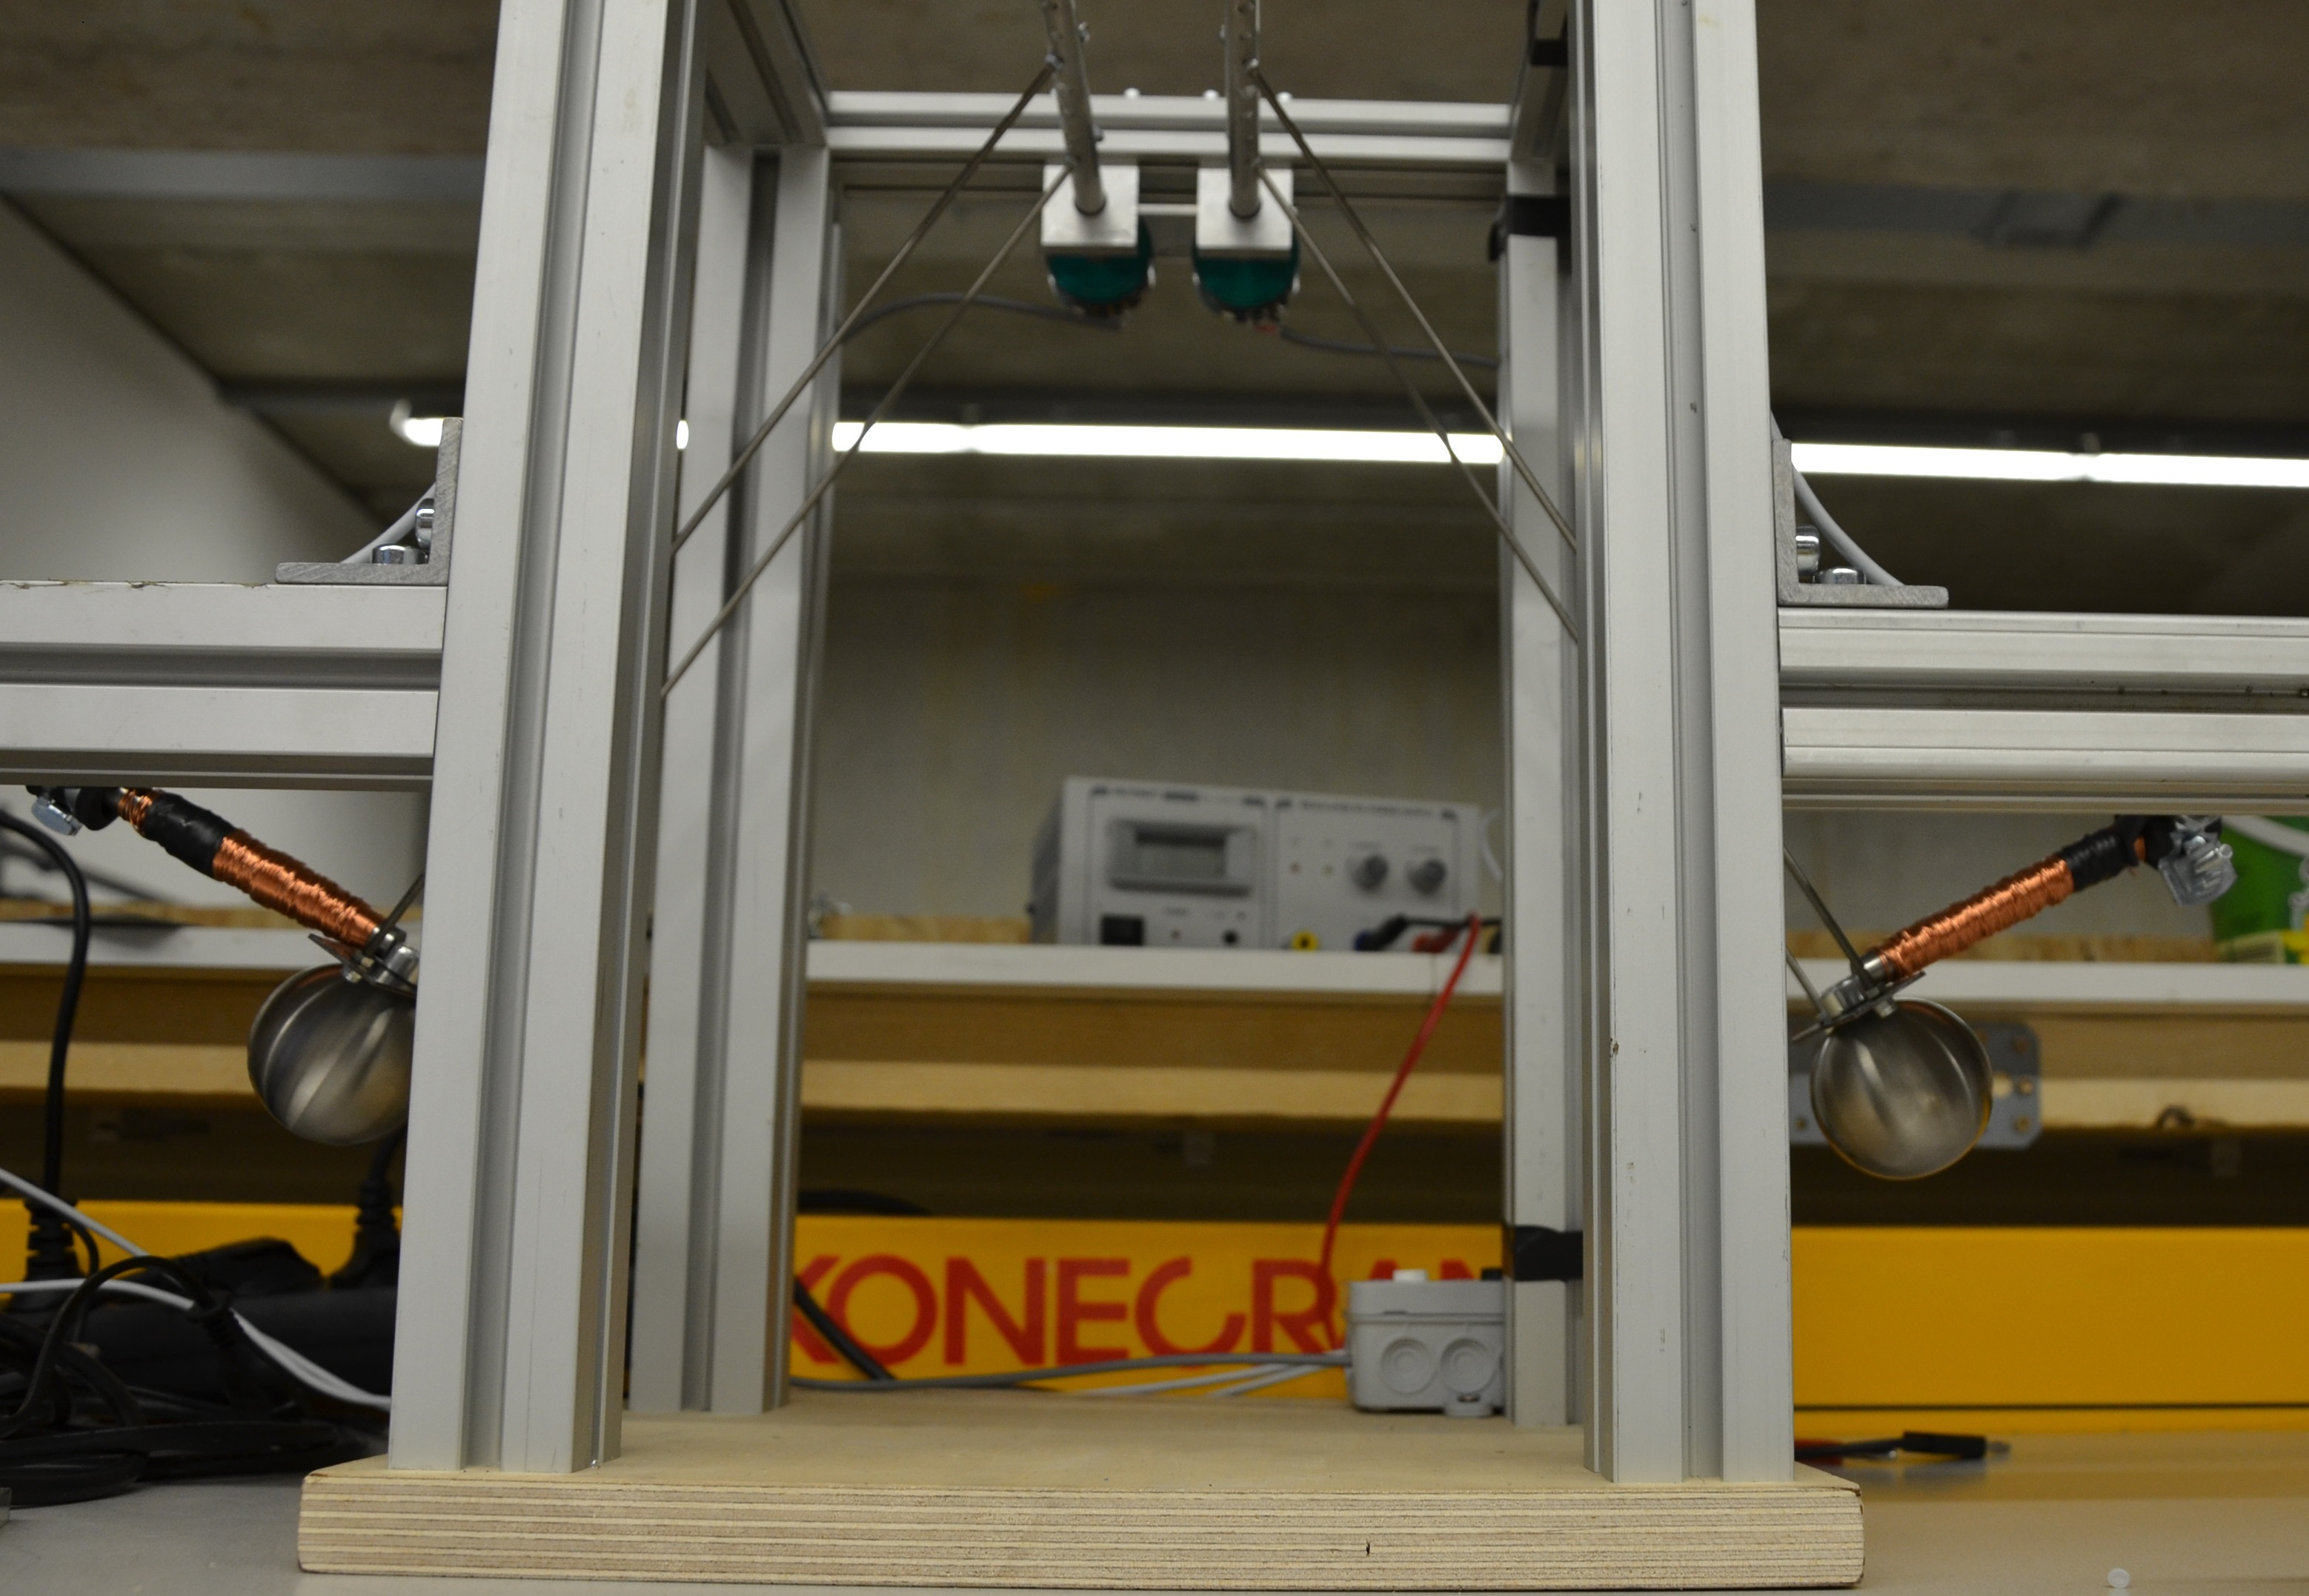
\includegraphics[width=.48\columnwidth]{007hollowspheredevice2}}  \quad
\subfloat[Coefficient of restitution of 2 mm silibeads]
{\label{fig:008esilibeads2mm2}%
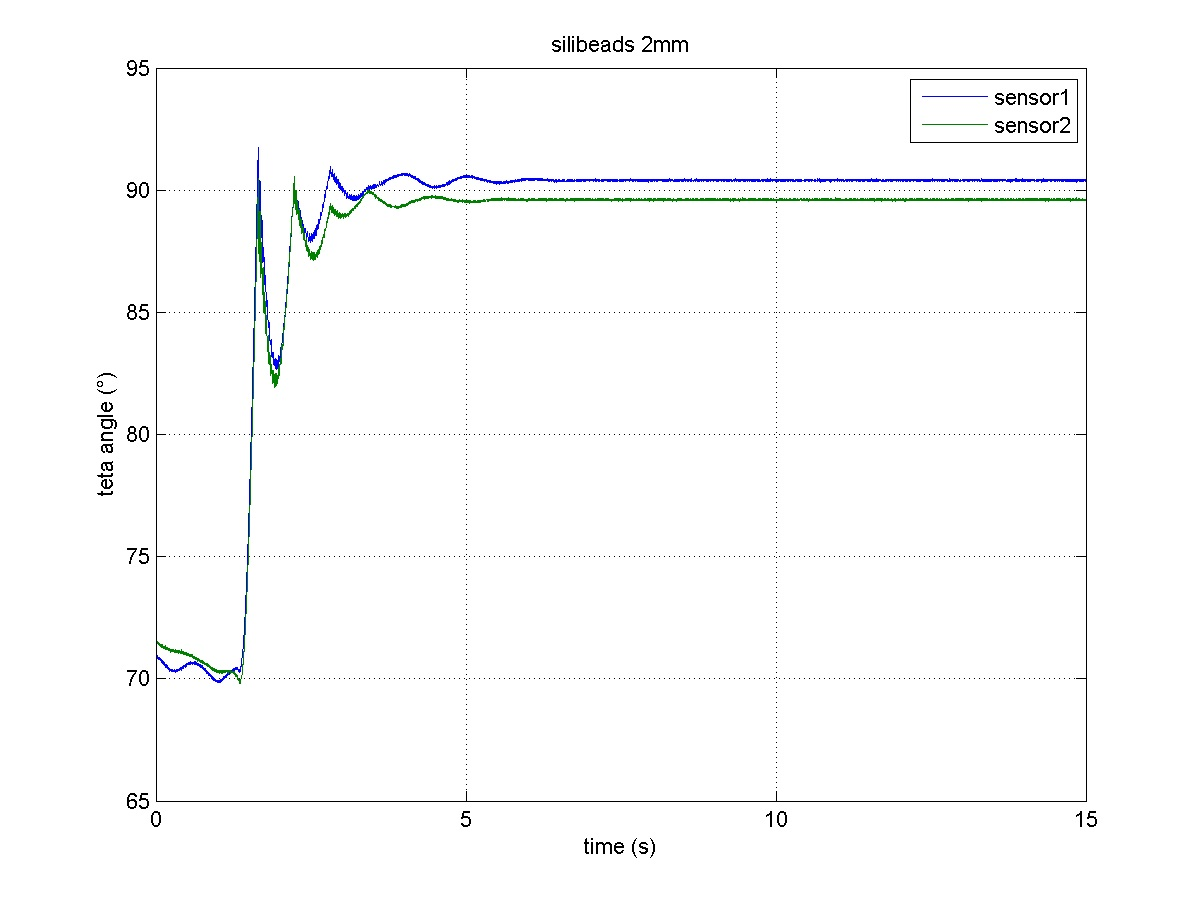
\includegraphics[width=.48\columnwidth]{008esilibeads2mm2}} \\
\caption[Hollow Spheres experiment]{Hollow Spheres experiment}
\label{fig:hollowspheres}
\end{figure}


Before start the spheres are kept at 40º from the vertical through magnetic rods, in order to avoid spin and torque when they are released.
After releasing the spheres move with a defined \ac{omega1}, calculated as the fraction of the angular displacement over time variation.
Then they collide and flee with an \ac{omega2}.\\

Now the results present little noise, as you can see in Figure \ref{fig:008esilibeads2mm2}.
Unfortunately the steel truss are transmitting vibration to the structure, I am trying to understand how much is the energy dissipation.\\

Soon I should receive a simulation script for this experiment.\\

%\subsubsection{HS}
%\label{subsubsection:hsexperiment}



%\subsubsection{HS simulation}
%\label{subsubsection:hssimulation}

